% !TEX root = main.tex
\section{Space Charge Effect Calibration}
\label{sec:sce-calib}

The build-up of slow-moving positive argon ions, produced by the continuous
cosmic-ray ionization of a surface LArTPC, distorts the nominally uniform drift
field. This causes \emph{spatial distortions} (a displacement of the
reconstructed position of ionization-electron clusters) and a position-dependent
change of the local field magnitude that modifies electron--ion recombination.
The calibration measures, throughout the active volume, the spatial distortion
field $\vec{D}(\vec{x})$ and the associated $\Delta\vec{E}/E_0$, stored as
voxelized maps (ROOT \texttt{TH3F}) for downstream reconstruction. The procedure
follows the MicroBooNE cosmic-muon method~\cite{ub_sce}, implemented in the
\texttt{CalibSCE} tool;\footnote{\url{https://github.com/mrmooney/CalibSCE}} it is
data-driven and proceeds in three steps that pin down the \emph{true}
entry/exit points of through-going muons at the boundaries and then the bulk
distortion, followed by the field derivation (Figure~\ref{fig:sce-threesteps}).

\paragraph{Common inputs and assumptions.}
The input is a sample of $t_0$-tagged cosmic-muon tracks ($\sim$200k),
classified by which faces their end points touch; the $t_0$ tag fixes the
absolute drift ($x$) coordinate. A dedicated SCE simulation map and a
drift-velocity model $v(E)$ are also used. The method assumes cosmic muons are
\emph{straight} over the drift, the \emph{anode is undistorted} (ionization
there barely drifts, giving an absolute reference), and the SCE is
approximately \emph{time-stable} (tracks need not share an event). The output is
a set of \texttt{TH3F} maps on a $\approx 10$~cm voxel grid, holding the
backward (reconstructed~$\rightarrow$~true) offsets $D_x,D_y,D_z$ and, after
Section~\ref{ssec:sce-efield}, the relative field distortions.

\begin{figure}[t]
  \centering
  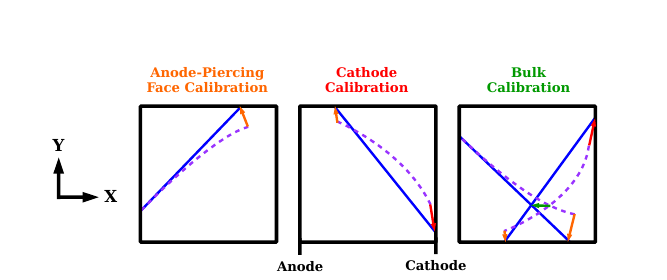
\includegraphics[width=0.82\linewidth]{figs/sce_threesteps.png}
  \caption{The three steps of the cosmic-muon SCE calibration, shown in the
  $Y$--$X$ plane of a TPC face (anode at left, cathode at right). Solid lines
  are reconstructed tracks; dashed lines are the inferred true trajectories.
  Step~1 calibrates the non-anode faces from anode-piercing tracks; Step~2
  calibrates the cathode; Step~3 uses near-crossing track pairs to measure the
  bulk distortion. Reproduced from the MicroBooNE SCE
  measurement~\cite{ub_sce}.}
  \label{fig:sce-threesteps}
\end{figure}

\subsection{Step 1 --- Anode-piercing face calibration}
\label{ssec:sce-anode}
\textbf{Assumption.} An anode-piercing track has no SCE distortion at the anode
end, so its other end marks the true crossing of one of the remaining five
faces.
\textbf{Input.} Anode-piercing $t_0$-tagged tracks; the SCE simulation map for
the transverse components.
\textbf{Algorithm.} For the non-anode end, the offset component
\emph{orthogonal} to the touched face is measured directly from the projected
distance of the track end to that face (adding $4.5$~cm in data to account for
the field-cage gap). The two in-face (transverse) components are then fixed
using ratios taken from the simulation, e.g.\ at the top face
\begin{equation}
\Delta x_{\rm reco}=\Delta y_{\rm reco}\,
\frac{\Delta x_{\rm sim}(x,z)}{\Delta y_{\rm sim}(x,z)},\qquad
\Delta z_{\rm reco}=\Delta y_{\rm reco}\,
\frac{\Delta z_{\rm sim}(x,z)}{\Delta y_{\rm sim}(x,z)} .
\end{equation}
The map is built in 2D voxels ($\approx 10$~cm) per face. Because the gap blinds
offsets below $4.5$~cm, the near-anode region ($x<100$~cm) is filled from
simulation, scaled to the data-driven measurements at larger $x$.
\textbf{Output.} Data-driven true entry/exit points (offset maps) on the top,
bottom, upstream, and downstream faces.

\subsection{Step 2 --- Cathode calibration}
\label{ssec:sce-cathode}
\textbf{Assumption.} Cathode offsets follow the simulated shape but are
normalized to the data measured at the top and bottom faces in Step~1.
\textbf{Input.} Cathode-piercing tracks; Step~1 results; the SCE simulation map.
\textbf{Algorithm.} A data-driven scale factor $S(y,z)$ is formed by
interpolating the top/bottom data-to-simulation ratios in $y$,
\begin{equation}
S(y,z)=F(y)\,\frac{\Delta y_{\rm reco}(y_{\rm top},z)}{\Delta y_{\rm sim}(y_{\rm top},z)}
+\big(1-F(y)\big)\,\frac{\Delta y_{\rm reco}(y_{\rm bot},z)}{\Delta y_{\rm sim}(y_{\rm bot},z)},
\quad F(y)=\frac{y-y_{\rm bot}}{y_{\rm top}-y_{\rm bot}},
\end{equation}
and applied to the simulated offsets at the cathode,
$\Delta x_{\rm reco}=S\,\Delta x_{\rm sim}$ (similarly for $y,z$). Built in 2D
voxels ($\approx 10$~cm).
\textbf{Output.} True entry/exit points at the cathode plane. After Steps~1--2,
the true end points of through-going tracks are known at all six faces.

\subsection{Step 3 --- TPC bulk calibration (crossing tracks)}
\label{ssec:sce-bulk}
\textbf{Assumption.} A through-going muon's true trajectory is the straight line
joining its two calibrated true face points; a single track is ambiguous, so
\emph{pairs} of near-crossing tracks are required to fix all three components
unambiguously.
\textbf{Input.} Through-going $t_0$-tagged tracks with calibrated end points
from Steps~1--2.
\textbf{Algorithm.} For each track the reconstructed points are compared with
the straight ``truth track''. For a pair of tracks, the near-crossing point of
the two truth tracks ($\vec{x}_{\rm true}$) and of the two reconstructed tracks
($\vec{x}_{\rm reco}$) are found; the correction vector at $\vec{x}_{\rm reco}$
is $\vec{D}=\vec{x}_{\rm true}-\vec{x}_{\rm reco}$. Both the truth-track and the
reconstructed-track members of a pair are required to approach within
$\approx 1$~cm of each other at the crossing. Per voxel ($\approx 10$~cm), the
offset is the \emph{median} of all contributing pairs, which also suppresses
multiple-Coulomb-scattering deviations from straightness. Gaps left by limited
track coverage are filled with a cubic spline followed by a
$3\times3\times3$ median filter, and complemented by the UV-laser calibration.
\textbf{Output.} The bulk spatial-distortion maps $D_x,D_y,D_z$ over the full
active volume (the backward, reconstructed~$\rightarrow$~true correction maps).

\subsection{Electric-field distortion calculation}
\label{ssec:sce-efield}
\textbf{Assumption.} The local drift velocity is set by the local field through
the measured $v(E)$ curve.
\textbf{Input.} The smoothed spatial-distortion map; the drift-velocity model
$v(E)$ (a polynomial fit, refined with a MicroBooNE drift-velocity
measurement).
\textbf{Algorithm.} The spatial map gives the local stretching/compression of
the drift path and hence the local drift velocity $v(x,y,z)$; inverting
$v(E)=v(x,y,z)$ numerically per voxel yields the local field magnitude, from
which the relative distortions $\Delta E_x/E_0,\Delta E_y/E_0,\Delta E_z/E_0$
and $\Delta|E|/E_0$ are computed.
\textbf{Output.} Electric-field distortion maps as \texttt{TH3F}, used to
correct recombination in the calorimetry.

\subsection{Implementation note for the present porting}
\label{ssec:sce-impl}
In the public \texttt{CalibSCE} code, only the \emph{bulk} step
(Section~\ref{ssec:sce-bulk}) is computed data-driven from the input tracks. The
face and cathode ``truthing'' of Steps~1--2 is instead obtained by correcting
the reconstructed end points with the SCE \emph{simulation} map (the
\texttt{output\_siminterp} file, via \texttt{getOffset}); the anode end uses only
a constant $t_0$/$x$ shift. Porting to SBND therefore requires either a trusted
SBND SCE simulation to anchor the end points, or a re-implementation of the
data-driven face/cathode steps; in both cases the geometry, drift field, $v(E)$
model, and the per-drift-volume structure of the two-anode SBND TPC must be
substituted.
